\documentclass[tikz,border=12pt]{standalone}
\usepackage[T1]{fontenc}
\usepackage{lmodern}
\usepackage{xcolor}
\usetikzlibrary{arrows.meta,backgrounds,calc,fit,positioning}

\definecolor{teacher}{HTML}{0F766E}
\definecolor{student}{HTML}{2563EB}
\definecolor{transfer}{HTML}{D97706}
\definecolor{distill}{HTML}{7C3AED}
\definecolor{ink}{HTML}{172033}
\definecolor{muted}{HTML}{566176}
\definecolor{paper}{HTML}{F8FAFC}

\begin{document}
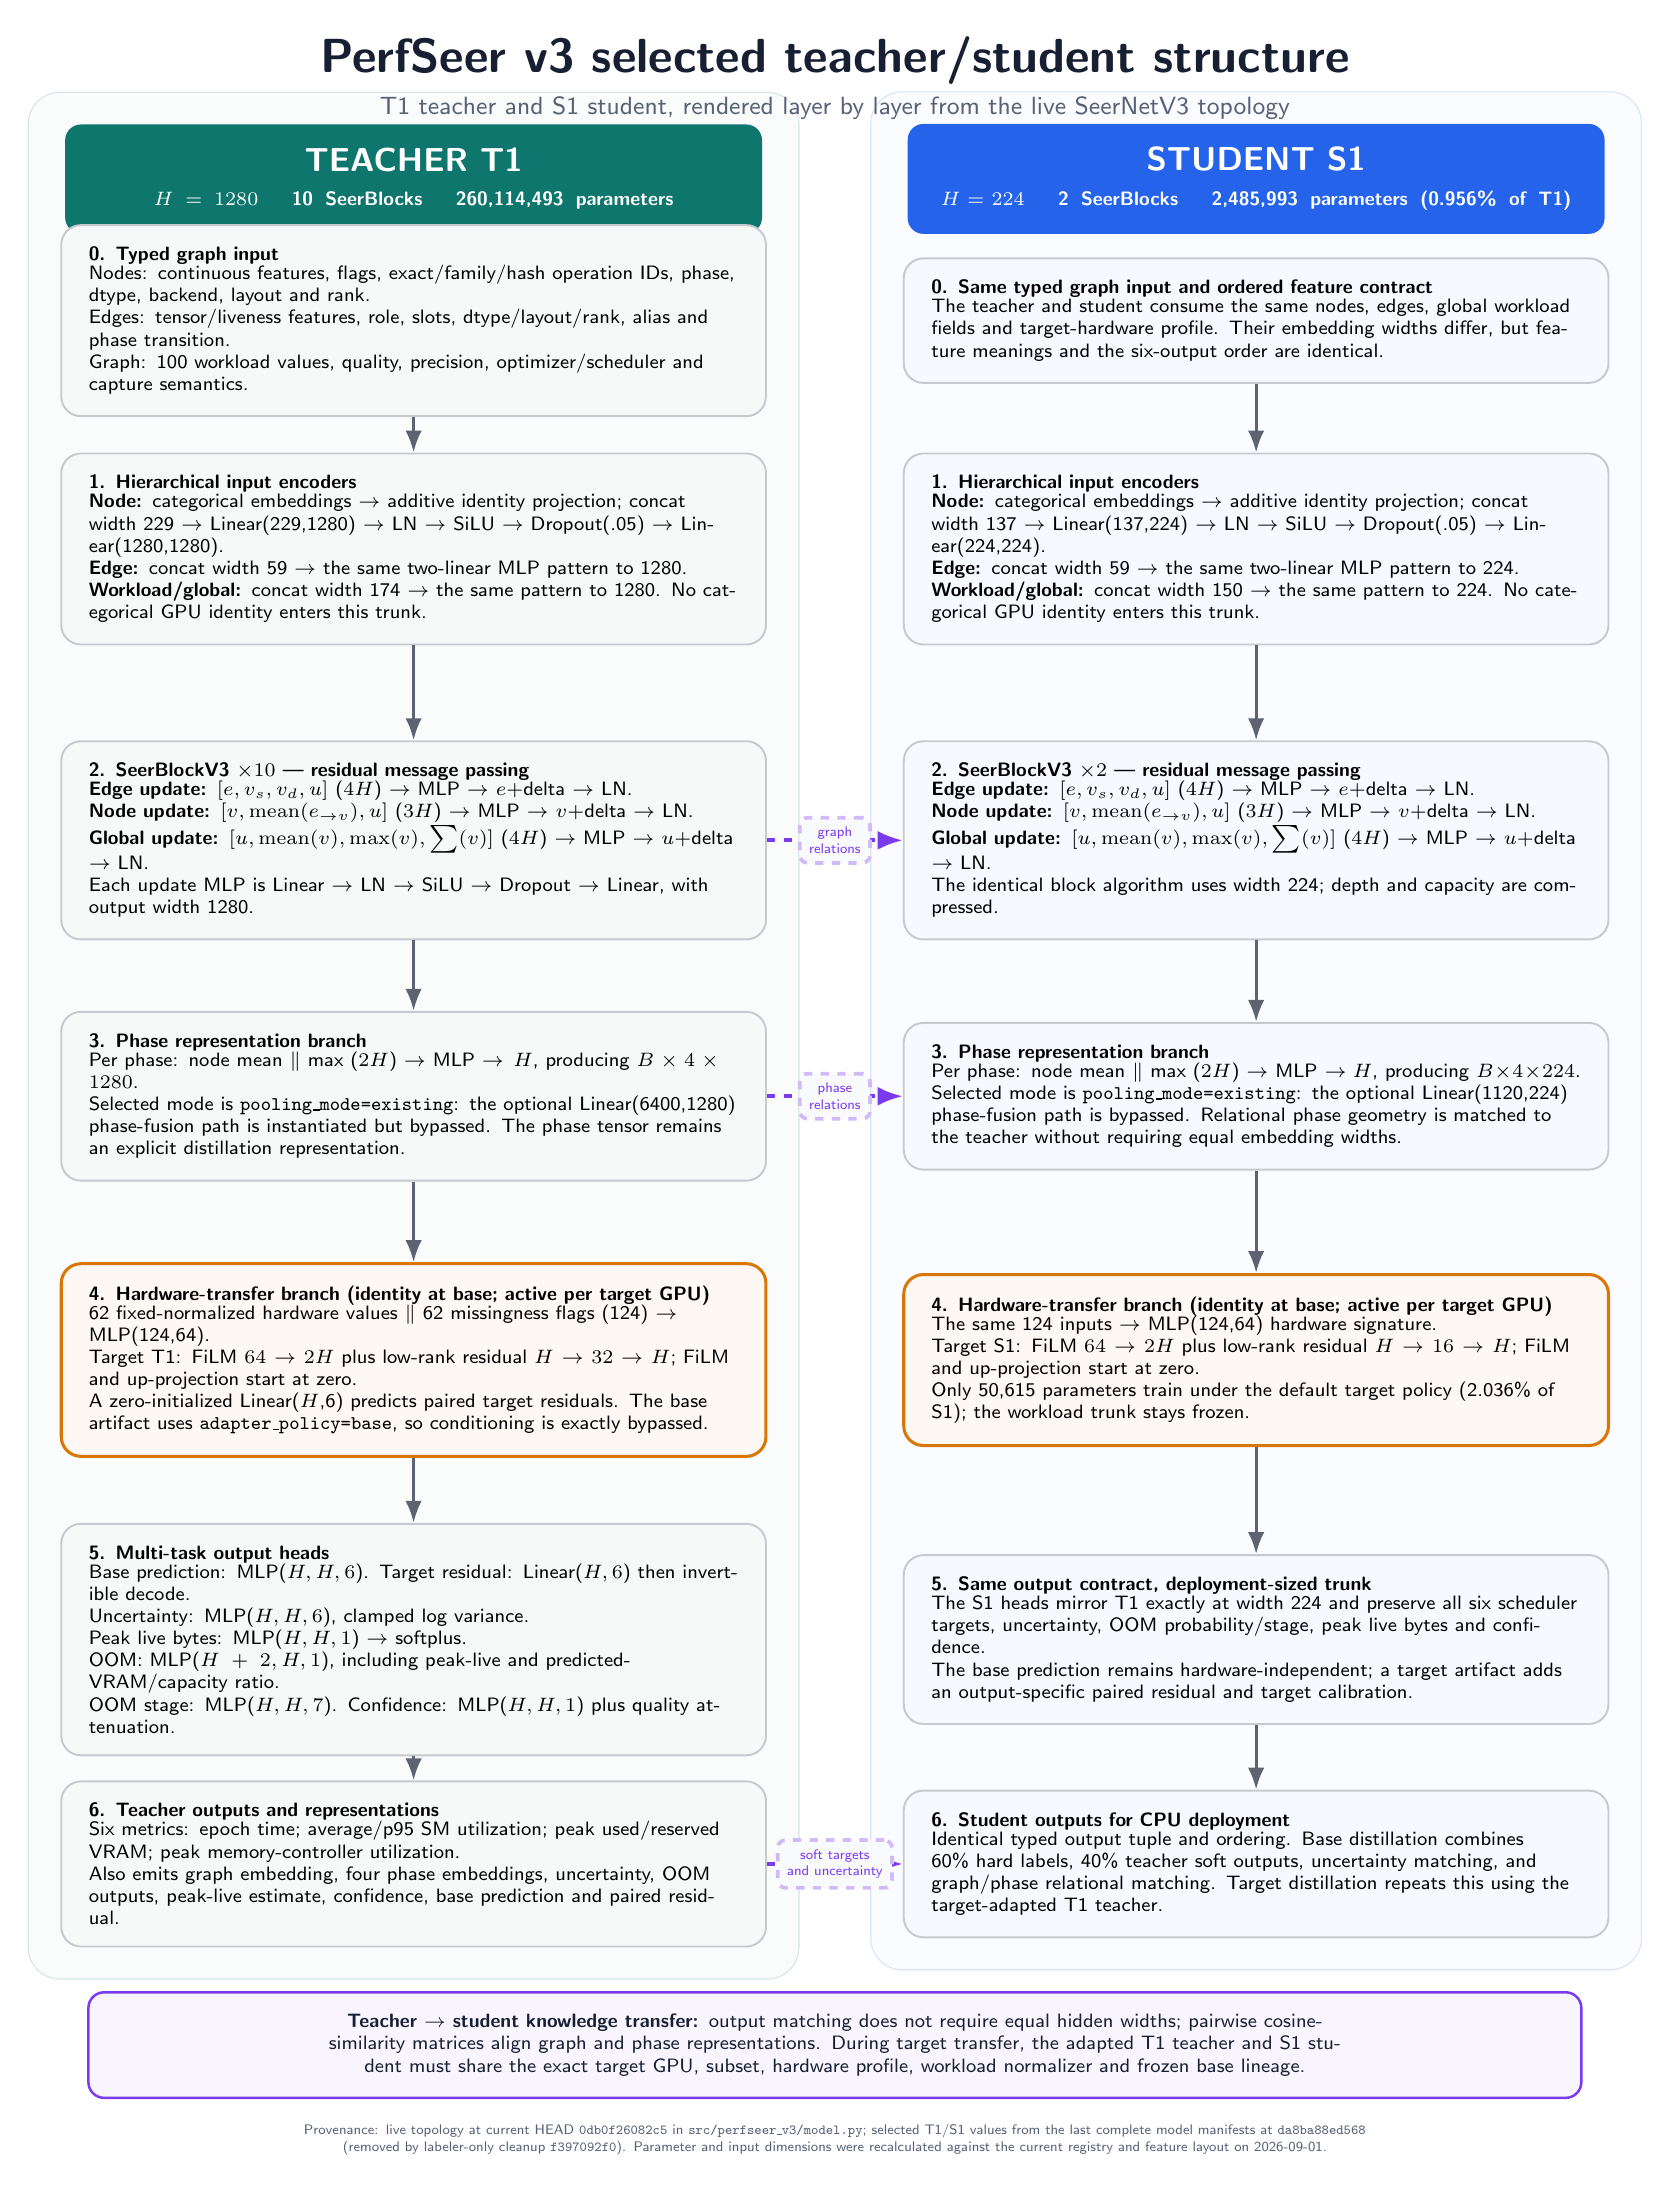
\begin{tikzpicture}[
  font=\sffamily,
  >={Latex[length=3mm]},
  layer/.style={
    rounded corners=2.5mm,
    draw=ink!24,
    line width=0.7pt,
    fill=white,
    text width=8.25cm,
    inner xsep=3.5mm,
    inner ysep=2.8mm,
    align=left,
    font=\sffamily\scriptsize
  },
  transferlayer/.style={layer,draw=transfer,line width=1.1pt,fill=transfer!5},
  flow/.style={-Latex,line width=1.1pt,draw=ink!70},
  distillation/.style={-Latex,dashed,line width=1.35pt,draw=distill},
  distilltag/.style={fill=paper,draw=distill!35,rounded corners=1mm,
    inner sep=1.2mm,font=\sffamily\tiny,text=distill,align=center},
  note/.style={font=\sffamily\tiny,text=muted,align=center}
]

\node[font=\sffamily\bfseries\LARGE,text=ink] at (5.35,2.65)
  {PerfSeer v3 selected teacher/student structure};
\node[font=\sffamily\small,text=muted,align=center] at (5.35,2.05)
  {T1 teacher and S1 student, rendered layer by layer from the live SeerNetV3 topology};

\node[rounded corners=2mm,fill=teacher,text=white,text width=8.25cm,
  inner sep=3mm,align=center,font=\sffamily\bfseries\large] (th) at (0,1.15)
  {TEACHER T1\\[-0.5mm]\scriptsize $H=1280$ \quad 10 SeerBlocks \quad 260,114,493 parameters};
\node[rounded corners=2mm,fill=student,text=white,text width=8.25cm,
  inner sep=3mm,align=center,font=\sffamily\bfseries\large] (sh) at (10.7,1.15)
  {STUDENT S1\\[-0.5mm]\scriptsize $H=224$ \quad 2 SeerBlocks \quad 2,485,993 parameters (0.956\% of T1)};

\node[layer,fill=teacher!4] (ti) at (0,-0.65) {%
  \textbf{0. Typed graph input}\\[-0.4mm]
  Nodes: continuous features, flags, exact/family/hash operation IDs, phase, dtype,
  backend, layout and rank.\\
  Edges: tensor/liveness features, role, slots, dtype/layout/rank, alias and phase transition.\\
  Graph: 100 workload values, quality, precision, optimizer/scheduler and capture semantics.};

\node[layer,fill=student!4] (si) at (10.7,-0.65) {%
  \textbf{0. Same typed graph input and ordered feature contract}\\[-0.4mm]
  The teacher and student consume the same nodes, edges, global workload fields and
  target-hardware profile. Their embedding widths differ, but feature meanings and the
  six-output order are identical.};

\node[layer,fill=teacher!4] (te) at (0,-3.55) {%
  \textbf{1. Hierarchical input encoders}\\[-0.4mm]
  \textbf{Node:} categorical embeddings $\rightarrow$ additive identity projection;
  concat width 229 $\rightarrow$ Linear(229,1280) $\rightarrow$ LN $\rightarrow$ SiLU
  $\rightarrow$ Dropout(.05) $\rightarrow$ Linear(1280,1280).\\
  \textbf{Edge:} concat width 59 $\rightarrow$ the same two-linear MLP pattern to 1280.\\
  \textbf{Workload/global:} concat width 174 $\rightarrow$ the same pattern to 1280.
  No categorical GPU identity enters this trunk.};

\node[layer,fill=student!4] (se) at (10.7,-3.55) {%
  \textbf{1. Hierarchical input encoders}\\[-0.4mm]
  \textbf{Node:} categorical embeddings $\rightarrow$ additive identity projection;
  concat width 137 $\rightarrow$ Linear(137,224) $\rightarrow$ LN $\rightarrow$ SiLU
  $\rightarrow$ Dropout(.05) $\rightarrow$ Linear(224,224).\\
  \textbf{Edge:} concat width 59 $\rightarrow$ the same two-linear MLP pattern to 224.\\
  \textbf{Workload/global:} concat width 150 $\rightarrow$ the same pattern to 224.
  No categorical GPU identity enters this trunk.};

\node[layer,fill=teacher!4] (tb) at (0,-7.25) {%
  \textbf{2. SeerBlockV3 $\times 10$ --- residual message passing}\\[-0.4mm]
  \textbf{Edge update:} $[e,v_s,v_d,u]$ ($4H$) $\rightarrow$ MLP $\rightarrow$ $e+$delta $\rightarrow$ LN.\\
  \textbf{Node update:} $[v,\mathrm{mean}(e_{\to v}),u]$ ($3H$) $\rightarrow$ MLP
  $\rightarrow$ $v+$delta $\rightarrow$ LN.\\
  \textbf{Global update:} $[u,\mathrm{mean}(v),\max(v),\sum(v)]$ ($4H$)
  $\rightarrow$ MLP $\rightarrow$ $u+$delta $\rightarrow$ LN.\\
  Each update MLP is Linear $\rightarrow$ LN $\rightarrow$ SiLU $\rightarrow$ Dropout
  $\rightarrow$ Linear, with output width 1280.};

\node[layer,fill=student!4] (sb) at (10.7,-7.25) {%
  \textbf{2. SeerBlockV3 $\times 2$ --- residual message passing}\\[-0.4mm]
  \textbf{Edge update:} $[e,v_s,v_d,u]$ ($4H$) $\rightarrow$ MLP $\rightarrow$ $e+$delta $\rightarrow$ LN.\\
  \textbf{Node update:} $[v,\mathrm{mean}(e_{\to v}),u]$ ($3H$) $\rightarrow$ MLP
  $\rightarrow$ $v+$delta $\rightarrow$ LN.\\
  \textbf{Global update:} $[u,\mathrm{mean}(v),\max(v),\sum(v)]$ ($4H$)
  $\rightarrow$ MLP $\rightarrow$ $u+$delta $\rightarrow$ LN.\\
  The identical block algorithm uses width 224; depth and capacity are compressed.};

\node[layer,fill=teacher!4] (tp) at (0,-10.50) {%
  \textbf{3. Phase representation branch}\\[-0.4mm]
  Per phase: node mean $\Vert$ max ($2H$) $\rightarrow$ MLP $\rightarrow H$,
  producing $B\times4\times1280$.\\
  Selected mode is \texttt{pooling\_mode=existing}: the optional
  Linear(6400,1280) phase-fusion path is instantiated but bypassed. The phase tensor
  remains an explicit distillation representation.};

\node[layer,fill=student!4] (sp) at (10.7,-10.50) {%
  \textbf{3. Phase representation branch}\\[-0.4mm]
  Per phase: node mean $\Vert$ max ($2H$) $\rightarrow$ MLP $\rightarrow H$,
  producing $B\times4\times224$.\\
  Selected mode is \texttt{pooling\_mode=existing}: the optional
  Linear(1120,224) phase-fusion path is bypassed. Relational phase geometry is matched
  to the teacher without requiring equal embedding widths.};

\node[transferlayer] (ta) at (0,-13.85) {%
  \textbf{4. Hardware-transfer branch (identity at base; active per target GPU)}\\[-0.4mm]
  62 fixed-normalized hardware values $\Vert$ 62 missingness flags (124)
  $\rightarrow$ MLP(124,64).\\
  Target T1: FiLM $64\rightarrow2H$ plus low-rank residual
  $H\rightarrow32\rightarrow H$; FiLM and up-projection start at zero.\\
  A zero-initialized Linear($H$,6) predicts paired target residuals. The base artifact
  uses \texttt{adapter\_policy=base}, so conditioning is exactly bypassed.};

\node[transferlayer] (sa) at (10.7,-13.85) {%
  \textbf{4. Hardware-transfer branch (identity at base; active per target GPU)}\\[-0.4mm]
  The same 124 inputs $\rightarrow$ MLP(124,64) hardware signature.\\
  Target S1: FiLM $64\rightarrow2H$ plus low-rank residual
  $H\rightarrow16\rightarrow H$; FiLM and up-projection start at zero.\\
  Only 50,615 parameters train under the default target policy (2.036\% of S1);
  the workload trunk stays frozen.};

\node[layer,fill=teacher!4] (thead) at (0,-17.40) {%
  \textbf{5. Multi-task output heads}\\[-0.4mm]
  Base prediction: MLP($H,H,6$). Target residual: Linear($H,6$) then invertible decode.\\
  Uncertainty: MLP($H,H,6$), clamped log variance.\\
  Peak live bytes: MLP($H,H,1$) $\rightarrow$ softplus.\\
  OOM: MLP($H+2,H,1$), including peak-live and predicted-VRAM/capacity ratio.\\
  OOM stage: MLP($H,H,7$). Confidence: MLP($H,H,1$) plus quality attenuation.};

\node[layer,fill=student!4] (shead) at (10.7,-17.40) {%
  \textbf{5. Same output contract, deployment-sized trunk}\\[-0.4mm]
  The S1 heads mirror T1 exactly at width 224 and preserve all six scheduler targets,
  uncertainty, OOM probability/stage, peak live bytes and confidence.\\
  The base prediction remains hardware-independent; a target artifact adds an
  output-specific paired residual and target calibration.};

\node[layer,fill=teacher!4] (to) at (0,-20.25) {%
  \textbf{6. Teacher outputs and representations}\\[-0.4mm]
  Six metrics: epoch time; average/p95 SM utilization; peak used/reserved VRAM;
  peak memory-controller utilization.\\
  Also emits graph embedding, four phase embeddings, uncertainty, OOM outputs,
  peak-live estimate, confidence, base prediction and paired residual.};

\node[layer,fill=student!4] (so) at (10.7,-20.25) {%
  \textbf{6. Student outputs for CPU deployment}\\[-0.4mm]
  Identical typed output tuple and ordering. Base distillation combines 60\% hard labels,
  40\% teacher soft outputs, uncertainty matching, and graph/phase relational matching.
  Target distillation repeats this using the target-adapted T1 teacher.};

\foreach \a/\b in {ti/te,te/tb,tb/tp,tp/ta,ta/thead,thead/to,
                    si/se,se/sb,sb/sp,sp/sa,sa/shead,shead/so}
  \draw[flow] (\a.south) -- (\b.north);

\draw[distillation] (tb.east) -- node[distilltag] {graph\\relations} (sb.west);
\draw[distillation] (tp.east) -- node[distilltag] {phase\\relations} (sp.west);
\draw[distillation] (to.east) -- node[distilltag] {soft targets\\and uncertainty} (so.west);

\node[rounded corners=2mm,draw=distill,fill=distill!5,line width=0.9pt,
  text width=18.4cm,inner sep=2.8mm,align=center,font=\sffamily\scriptsize,
  text=ink] (loss) at (5.35,-22.55) {%
  \textbf{Teacher $\rightarrow$ student knowledge transfer:}
  output matching does not require equal hidden widths; pairwise cosine-similarity
  matrices align graph and phase representations. During target transfer, the adapted
  T1 teacher and S1 student must share the exact target GPU, subset, hardware profile,
  workload normalizer and frozen base lineage.};
\node[note,text width=19.3cm] at (5.35,-23.75) {%
  Provenance: live topology at current HEAD \texttt{0db0f26082c5} in
  \texttt{src/perfseer\_v3/model.py}; selected T1/S1 values from the last complete model
  manifests at \texttt{da8ba88ed568} (removed by labeler-only cleanup
  \texttt{f397092f0}). Parameter and input dimensions were recalculated against the
  current registry and feature layout on 2026-09-01.};

\begin{scope}[on background layer]
  \node[fit=(th)(ti)(te)(tb)(tp)(ta)(thead)(to),rounded corners=4mm,
    fill=teacher!2,draw=teacher!18,inner sep=4mm] {};
  \node[fit=(sh)(si)(se)(sb)(sp)(sa)(shead)(so),rounded corners=4mm,
    fill=student!2,draw=student!18,inner sep=4mm] {};
\end{scope}

\end{tikzpicture}
\end{document}
